\documentclass[10pt]{article}
\usepackage[a4paper,margin=1.9cm]{geometry}
\usepackage{amsmath,amssymb}
\usepackage{graphicx}
\graphicspath{{../}{./}}
\usepackage{float}
\usepackage[dvipsnames]{xcolor}
\usepackage{enumitem}
\usepackage{titlesec}
\usepackage[hidelinks]{hyperref}

% --- compact layout ---
\setlist[itemize]{leftmargin=1.35em,itemsep=1pt,topsep=2pt,parsep=0pt}
\setlength{\parindent}{0pt}
\setlength{\parskip}{3pt}
\titlespacing*{\section}{0pt}{6pt}{3pt}
\titlespacing*{\subsection}{0pt}{4pt}{2pt}
\titleformat{\section}{\normalfont\large\bfseries\color{RoyalBlue}}{\thesection.}{0.5em}{}
\titleformat{\subsection}{\normalfont\bfseries}{}{0em}{}

\newcommand{\code}[1]{\texttt{\small #1}}
\newcommand{\file}[1]{\textcolor{RoyalBlue}{\texttt{\small #1}}}

% \docheader{title}{subtitle}
\newcommand{\docheader}[2]{%
  \begin{center}
    {\LARGE\bfseries #1}\\[2pt]
    {\small #2}
  \end{center}
  \vspace{-4pt}\hrule\vspace{6pt}
}

\begin{document}

\docheader{Adora --- Piecewise-Linear Formal Solver}%
{As-built notes \quad$\cdot$\quad Ivan Milic \quad$\cdot$\quad 2026-09-20 \quad$\cdot$\quad session summary}

Upgraded the polarised formal solver from piecewise-constant (DELO) to \textbf{piecewise-linear}
(DELO-linear). New code lives in \file{formal\_solvers/}; the old \file{vector\_formal\_solver.py} is
untouched. \code{delo\_linear\_fs} is a \textbf{drop-in} for \code{delo\_constant\_fs} (same signature
\code{(dz, I\_start, emis, opac)}) --- only the physics changed --- and is now wired into
\file{vector\_response\_fn.py} (see \S4).

\subsection*{1. The physics change}
The DELO machinery (\code{stokes\_K}, $K'=K/K_{00}-I$, $\Phi_k$, $\Phi_{k+1}$, \code{jnp.linalg.solve},
\code{fori\_loop}) is unchanged. Only the two source/coupling weights change: the constant
$0.5\,F_k$ trapezoid becomes the linear-source weights (Olson \& Kunasz 1987). With $u=\Delta\tau$,
$E=e^{-u}$, $w_0=1-E$, $w_1=1-(1+u)E$:
\[
\psi_a = \frac{w_1}{u}\ \text{(upwind: }K'_m,\eta_m),\qquad
\psi_b = w_0 - \frac{w_1}{u}\ \text{(local: }K',\eta),\qquad \psi_a+\psi_b = w_0 .
\]
The sum is unchanged (constant-source limit identical), but the weights redistribute correctly toward
the local point as a layer becomes optically thick --- which is where the constant scheme's staircase
error lives.

\subsection*{2. The gradient hazard (the reason to be careful)}
$\psi = w_1/u$ is $0/0$ as $u\to0$: the \emph{value} is finite but its \textbf{autodiff derivative is
NaN}, and small $u$ is exactly the top layers and line wings. Fix: a Taylor expansion to $O(u^3)$ below
\code{eps=1e-3}, applied with the double-\code{where} (\code{safe=where(u<eps,1,u)}) so the discarded
branch never divides by zero. This is the make-or-break detail; it is verified below.

\subsection*{3. Validation (\file{formal\_solvers/validate\_linear.py})}
\textbf{Gradients (clean).} \code{jacrev(delo\_linear\_fs)} is finite even at $\Delta\tau=8\times10^{-5}$
(guard works) and matches finite differences ($\sim$\code{1e-8} at thick layers; the lone \code{5.8e-4}
is FD noise where the sensitivity is $\approx0$). Full-RT \code{jacrev} w.r.t.\ $T$ is finite,
$\max|\partial I/\partial T|=2.15\times10^{-3}$ (matches the known f64 value).

\textbf{Forward vs Lightweaver (FAL, fine grid).} Linear $\approx$ constant (linear slightly better in
$Q,U,V$; tie in $I$); \emph{both} sit $\sim$5--7\% from Lightweaver, a residual set by the opacity physics
(Fe-only partition functions, simplified continuum), \textbf{not} the solver.

\textbf{Coarse grid (isolates the solver: same opacity code, fine-grid linear = truth).} This is the
payoff --- as layers thicken, linear clearly beats constant:
\smallskip

\begin{tabular}{@{}l r r@{}}
\hline
\textbf{grid} & \textbf{linear} & \textbf{constant}\\
\hline
\code{skip=4}\ \ (21 layers) & \textbf{3.6e-2} & 1.4e-1\ \ ($\sim$4$\times$ worse)\\
\code{skip=8}\ \ (11 layers) & \textbf{2.6e-1} & 5.2e-1\ \ ($\sim$2$\times$ worse)\\
\hline
\end{tabular}
\smallskip

\begin{center}
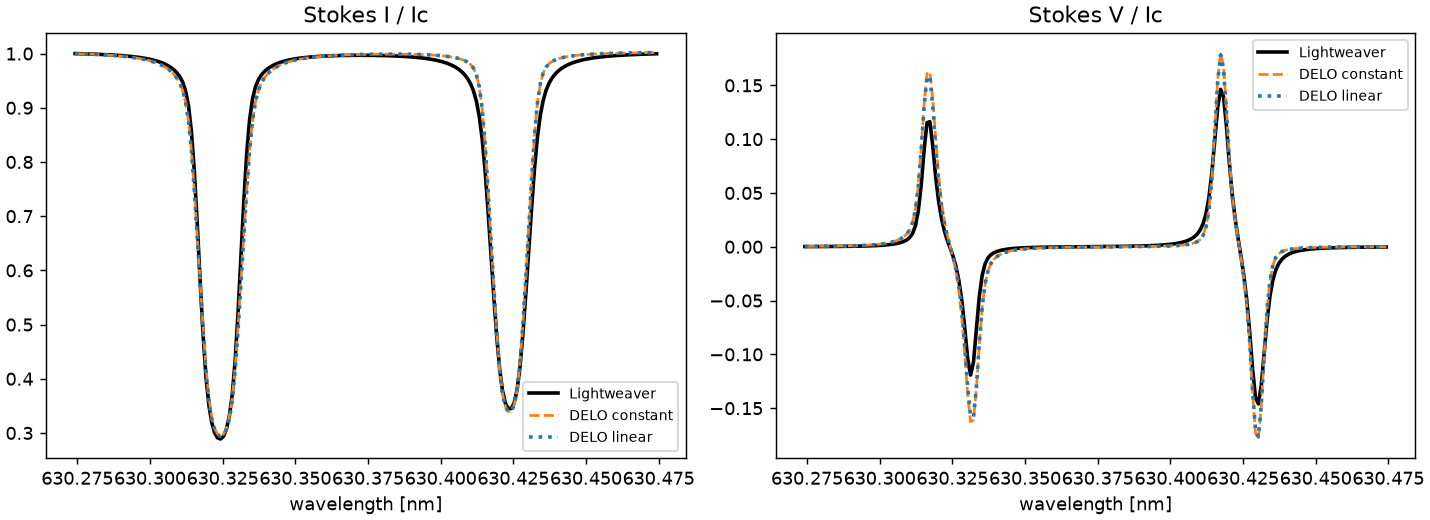
\includegraphics[width=0.92\linewidth]{validate_linear.png}\\[2pt]
{\small\itshape FAL-C fine grid: Lightweaver vs DELO constant vs linear (normalised by own continuum);
constant and linear overlie, and the offset from Lightweaver is opacity physics, not the solver.}
\end{center}

\subsection*{4. Wired in, and a scalar twin}
\code{delo\_linear\_fs} is now the solver used by \file{vector\_response\_fn.py} (\code{lte\_polarised\_rt}),
so the whole synth/inversion path runs on it. A matching \textbf{scalar} solver
\code{formal\_solvers/scalar\_formal\_solver\_linear.linear\_fs} was added the same way (identical linear
weights + small-$\Delta\tau$ guard) and wired into \file{response\_fn.py} (\code{lte\_rt}); it behaves the
same --- $\sim$free on the fine grid, and an even larger coarse-grid gain, since the old single-point
\code{nearest\_fs} blows up ($\sim$\code{2.4e4} at skip=8) where linear stays $\sim$0.3. f64 throughout;
files uncommitted.

\end{document}
